 \documentclass{beamer}
\mode<presentation>
\usepackage{amsmath}
\usepackage{amssymb}
%\usepackage{advdate}
\usepackage{graphicx}
\usepackage{adjustbox}
\usepackage{subcaption}
\usepackage{enumitem}
\usepackage{multicol}
\usepackage{mathtools}
\usepackage{listings}
\usepackage{url}
\def\UrlBreaks{\do\/\do-}
\usetheme{Boadilla}
\usecolortheme{lily}
\let\vec\mathbf
\setbeamertemplate{footline}
{
  \leavevmode%
  \hbox{%
  \begin{beamercolorbox}[wd=\paperwidth,ht=2.25ex,dp=1ex,right]{author in head/foot}%
    \insertframenumber{} / \inserttotalframenumber\hspace*{2ex} 
  \end{beamercolorbox}}%
  \vskip0pt%
}
\setbeamertemplate{navigation symbols}{}

\providecommand{\nCr}[2]{\,^{#1}C_{#2}} % nCr
\providecommand{\nPr}[2]{\,^{#1}P_{#2}} % nPr
\providecommand{\mbf}{\mathbf}
\providecommand{\pr}[1]{\ensuremath{\Pr\left(#1\right)}}
\providecommand{\qfunc}[1]{\ensuremath{Q\left(#1\right)}}
\providecommand{\sbrak}[1]{\ensuremath{{}\left[#1\right]}}
\providecommand{\lsbrak}[1]{\ensuremath{{}\left[#1\right.}}
\providecommand{\rsbrak}[1]{\ensuremath{{}\left.#1\right]}}
\providecommand{\brak}[1]{\ensuremath{\left(#1\right)}}
\providecommand{\lbrak}[1]{\ensuremath{\left(#1\right.}}
\providecommand{\rbrak}[1]{\ensuremath{\left.#1\right)}}
\providecommand{\cbrak}[1]{\ensuremath{\left\{#1\right\}}}
\providecommand{\lcbrak}[1]{\ensuremath{\left\{#1\right.}}
\providecommand{\rcbrak}[1]{\ensuremath{\left.#1\right\}}}
\theoremstyle{remark}
\newtheorem{rem}{Remark}
\newcommand{\sgn}{\mathop{\mathrm{sgn}}}
\providecommand{\abs}[1]{\vert#1\vert}
\providecommand{\res}[1]{\Res\displaylimits_{#1}} 
\providecommand{\norm}[1]{\lVert#1\rVert}
\providecommand{\mtx}[1]{\mathbf{#1}}
\providecommand{\mean}[1]{E[ #1 ]}
\providecommand{\fourier}{\overset{\mathcal{F}}{ \rightleftharpoons}}
%\providecommand{\hilbert}{\overset{\mathcal{H}}{ \rightleftharpoons}}
\providecommand{\system}[1]{\overset{\mathcal{#1}}{ \longleftrightarrow}}
%\providecommand{\system}{\overset{\mathcal{H}}{ \longleftrightarrow}}
	%\newcommand{\solution}[2]{\vec{Solution:}{#1}}
%\newcommand{\solution}{\noindent \vec{Solution: }}
\providecommand{\dec}[2]{\ensuremath{\overset{#1}{\underset{#2}{\gtrless}}}}
\newcommand{\myvec}[1]{\ensuremath{\begin{pmatrix}#1\end{pmatrix}}}


\lstset{
%language=C,
frame=single, 
breaklines=true,
columns=fullflexible
}
\lstset{
  language=C,
  basicstyle=\ttfamily\footnotesize,
  keywordstyle=\color{blue}\bfseries,
  commentstyle=\color{gray}\itshape,
  stringstyle=\color{orange},
  numbers=left,
  numberstyle=\tiny\color{gray},
  breaklines=true,
  frame=single,
  showstringspaces=false,
  tabsize=4,
  captionpos=b
}
\numberwithin{equation}{section}
\lstset{
  language=Python,
  basicstyle=\ttfamily\small,
  keywordstyle=\color{blue},
  stringstyle=\color{orange},
  numbers=left,
  numberstyle=\tiny\color{gray},
  breaklines=true,
  showstringspaces=false
}

\title{Problem 12.217}
\author{Sujal Rajani}

\date{\today} 
\begin{document}

\begin{frame}
\titlepage
\end{frame}

\section{Question}
\begin{frame}{Question}
\textbf{Question }:
Given the surface
\[
x^2 + \frac{y^2}{4} + \frac{z^2}{9} = 3,
\]
find the directional derivative at \(P(1,2,3)\) in the direction of the vector $\vec{P}$, where \(O\) is the origin.

\end{frame}
\begin{frame}{Solution}
\textbf{SOLUTION}
\subsection*{Step 1: Theorem for Directional Derivative}
\\
we represent the partial derivative as :
\\
\begin{align*}
    \frac{\partial f}{\partial x}=f_x(x,y)
\end{align*} 
\\
 the directional derivative of \(f(x, y)\) in the direction of the unit vector $\vec{u}$ =  \myvec{a\\ b} is
\[
D_{\mathbf{u}} f(x, y) = f_x(x, y)a + f_y(x, y)b,
\]
and in three dimensions,
\[
D_{\mathbf{u}} F(x, y, z) = \vec{\nabla F(x, y, z)}^\top  \vec{u},
\]
where $\vec{\nabla F}$ is the gradient of \(F\).
     \end{frame}
     \begin{frame}{ Step-by-Step Calculation}    
\subsection*{Step 2: Find the Gradient}

Let
\[
F(x, y, z) = x^2 + \frac{y^2}{4} + \frac{z^2}{9}.
\]
Compute the gradient:
\[
\vec{\nabla F} = \left( \frac{\partial F}{\partial x}, \frac{\partial F}{\partial y}, \frac{\partial F}{\partial z} \right)^\top
= \myvec{2x& \frac{y}{2}& \frac{2z}{9}}^\top
\]

At \(P(1,2,3)\):
\begin{align*}
\vec{\nabla F(1,2,3)} =  \myvec{2&1&\frac{2}{3}}^\top
\end{align*}
     \end{frame}
     \begin{frame}{ Step-by-Step Calculation}    
\textbf{Step 3: Unit Direction Vector}
\\
The position vector from the origin to the point \(P(1,2,3)\) is
\begin{align*}
    \vec{P}= \myvec{1\\2\\3}
\end{align*}
To get the unit vector,
\begin{align*}
||\vec{P}||^2 =\vec{P}^\top\vec{P}=1^2 + 2^2 + 3^2 = {14} 
\\
\vec{\hat{P}}=\dfrac{\vec{P}}{||\vec{P}||}
\end{align*}

So,
\[
\vec{\hat{P}} = \left(\frac{1}{\sqrt{14}}, \frac{2}{\sqrt{14}}, \frac{3}{\sqrt{14}}\right)^\top
\]

     \end{frame}
     \begin{frame}{ Step-by-Step Calculation}    
\subsection*{Step 4: Directional Derivative Formula and Calculation}

By the theorem :
\[
D_{\mathbf{u}} F = \vec{{\nabla F}}^\top  \vec{\hat{P}}
\]
\[
=  \frac{2}{\sqrt{14}} + \frac{2}{\sqrt{14}} +  \frac{2}{\sqrt{14}}
\]
\[
= \frac{6}{\sqrt{14}}
\]

\subsection*{Final Answer}
\[
\boxed{ \frac{6}{\sqrt{14}} }
\]
     \end{frame}
    
       \begin{frame}[fragile]
    \begin{figure}[H]
    \centering
    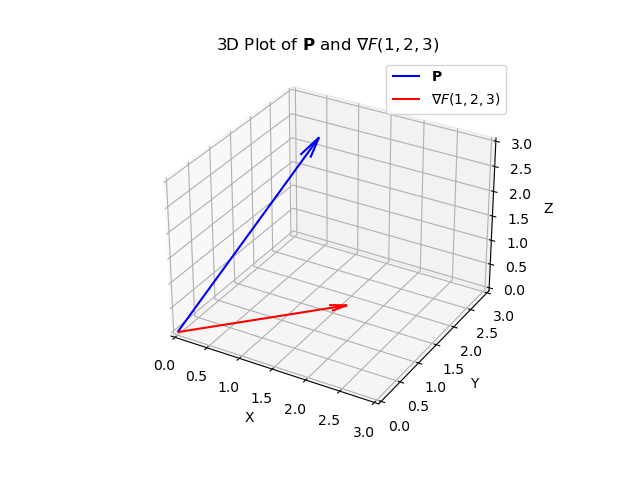
\includegraphics[width = 0.6\columnwidth]{../figs/img.png}
    \caption*{}
    \label{figs}
\end{figure}
\end{frame}

\end{document}